\documentclass{article}

\begin{document}

Estimation of the hand gesture from the muscle activity of the forearm using sEMG sensors is a challenging subject of machine learning due to multiple complexities.
\begin{itemize}
    \item The sEMG sensor do not get all the muscle activity of the forearm due to their limitation to the surface of the arm (for non-invasive purpose).
    \item The resolution of the sEMG electrodes is quite low compared to all the combined muscle activity that the forearm shows when doing complex had gestures (The forearm by itself has 20 independent muscles).
    \item The hand is the part of human anatomy which has the most degrees of liberty (27 DOF).
    \item Training a machine learning algorithm requires a ground truth which is not directly available when the subject has a missing hand.
\end{itemize}

There exist nevertheless a lot of techniques that enable to estimate the posture (still position) and the gesture (movement) of the hand based only on sEMG signals taken from different points of the forearm.


\subsection{Applications}

The main application of this kind of estimation is to control myoelectric hand prosthesis for people having a missing hand in order to give them abilities that are not available or difficult to achieve with an amputated hand. It is however not the only application of such predictions. A non-exhaustive list of the applications is given below

\begin{itemize}
    \item Myoelectric hand prosthesis control:  The robotic arm must be able to perform series of real life motions of the have each of its finger independently driven.
    \item Virtual reality control:  The aim is to have the user seeing both its hands, inside the virtual reality, synchonized with its real hands. This kind of technology already exist \cite{ref:oculus1} but using cameras to estimate the hand position which requires the user to keep its hands in front of the headset.
    \item Sign language automatic traduction \cite{ref:signLang2, ref:signLang3}: The device must be able to recognize a series of postures which can be translated into spoken language to enable mute people to be understood easily by everyone.
\end{itemize}


	
\subsection{Types of hand gesture estimation}

The two kinds of machines learning predictions algorithms are called \textit{classification} and \textit{regression}. They both have applications in estimation of hand gestures. For classification, it consists in having a set of predefined postures that can be recognized. The number of such postures is quite low in every current studies which is often not sufficient for most of the applications. It is however the easiest kind of estimation that can be done on this kind of data. For regression, the algorithm must be able to estimate as many DOF as possible independently in order to give a more natural feeling to the estimation. This kind of prediction is way more difficult to realise as the combined gestures of all fingers of the hand are producing complex muscular activity where it is not possible to easily isolate the signal related to each finger. That is why, to this day, most of the studies on hand gesture estimation based on sEMG signals have concentrated on posture classification. 


\subsection{Preprocessing}

Before extracting any kind of information from the raw sEMG signal, some preprocessing must be made in order to highlight the important information. The usual preprocessing pipeline contains filtering, signal segmentation and domain transformation.

\subsubsection{Filtering}

The first preprocessing that should be applied on the signal is filtering. Its purpose is to reduce the noise in the data. \cite{ref:classification3, ref:classification4}


\subsubsection{signal segmentation}

Also called windowing, this enables to cut the complete signal in a set of short duration signals that all have the same length which allows easier classification. There are two types of windowing methods: overlapping segmentation and disjoint segmentation (also called sliding segmentation \cite{ref:classification1}). In overlapping segmentation, the increment of time between the start of a segment and the next one is smaller than the duration of the segments. In disjoint segmentation, this increment is equal to the duration of the window\cite{ref:classification3, ref:classification4}. In the literature, size of the window goes between 200ms and 750ms.

\subsubsection{Domain transformation}

When collecting the sEMG from a patient, the raw signal is given in the time domain. This representation of the data is the easiest to get and can already show some information but it is not sufficient to extract all the relevant features. There exist two additional representation of the sEMG signal, being the frequency domain and the time-frequency domain, that are computed from the time domain to highlight different features.

\paragraph{Time domain}
This domain gives the time on the horizontal axis and the amplitude of the signal of the vertical axis. It can be used to find frequencies of the signal and duration. \cite{ref:classification4}

\paragraph{Frequency domain}
Instead of having the time on the horizontal axis, this domain has the complete range of possible frequencies of the signal while the vertical axis gives the amplitude of each of these frequencies. This representation does not show the evolution of the signal in the time. It can be computed from the time domain using power spectral density (PSD).\cite{ref:classification4}

\subparagraph{PSD computation}
The power spectral density (PSD) is computed as the Fourier transform of the auto-correlation function \cite{ref:masterThesisCedricSimar}. The auto-correlation function gives the correlation of a signal with itself in a shifted time position. This function is given in equation \ref{eq:acf} where $x(t)$ gives the amplitude of the signal at time $t$.

\begin{equation}
    R(\tau) = \int_{-\infty}^{\infty}x(t) x(t + \tau) dt
    \label{eq:acf}
\end{equation}

The formula of the PSD function is then given in equation \ref{eq:psd},

\begin{equation}
    F(R(\tau)) = \int_{-\infty}^{\infty} R(\tau) e^{-i \omega \tau} d \tau
    \label{eq:psd}
\end{equation}

where $\omega = 2 \pi f$ is the angular frequency for a frequency $f$ of the signal and $i=\sqrt{-1}$. The PSD function is the decomposition in sinusoïds of the auto-correlation function.

To compute the PSD on sample signals, we use the Welch's method (also called weighted overlapped segment averaging (WOSA) method or periodogram averaging method) \cite{ref:psd1, ref:psd2}. This algorithm can be described by the following pseudo-code \cite{ref:psd2}.
\begin{enumerate}
    \item Cut the signal into K overlapping segments (also called batches) of the same length
    \item On each segment, compute a discrete Fourier transform (DFT) for a specific frequency
    \item Find the modified periodogram of each segment from its DFT
    \item Average the periodogram values
\end{enumerate}

\paragraph{Time-Frequency domain}

This domain allows to study the signal frequency-domain and time-domain at the same time \cite{ref:wikiTimeFreqDomain}. There exist multiple representation of this domain. For the analysis of EMG signal, the Wavelet transform can be used \cite{ref:timeFreqDomain}. As an example, a study \cite{ref:timeFreqDomain} on the EMG signal of the while walking has used the representation in figure \ref{fig:timeFreqDomain} of the time-frequency domain to analyse its signals. A single figure gives the evolution of the frequency during a full step (gait cycle).

\begin{figure}[H]
    \centering
    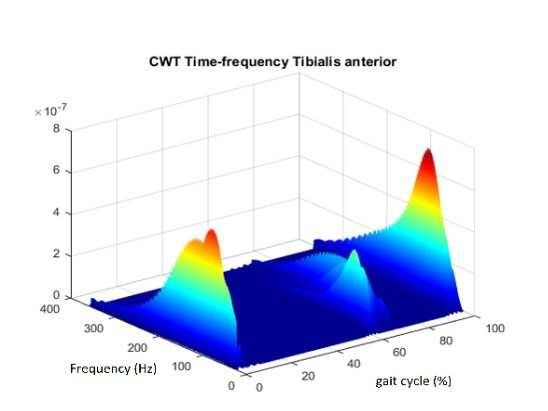
\includegraphics[width=10cm]{images/timeFreqDomainExample.png}
    \caption{Example of the representation of the time-frequency domain with wavelet coefficients given in colors \cite{ref:timeFreqDomain}}
    \label{fig:timeFreqDomain}
\end{figure}


Because of the high need in computational power to compute the time-domain frequency, it is not used in practise in any therapeutic device. \cite{ref:classification4}.



\subsection{Feature Ingineering}
A series of features that are known to provide good classification support can be extracted from the two domains that are considered for therapeutic device. From the time domain, we can find the mean absolute value (MAV), the waveform length (WL), the wavelet transform (WT), the Willison amplitude (WAMP), the slope sign change (SSC), the zero-crossings (ZC), the root meam square (RMS), the integral of the EMG (IEMG), the mathematical moments (MM), the simple square integral (SSI) and the variance of the EMG (VAR). From the frequency domain, we can extract the autoregressive coefficients (AR), the frequency median (FMD), the modified median frequency (MMDF) and the modified frequency mean (MMNF). Some of this feature can, alone, already give some possibilities of classification but its only by combining multiple features that we get the highest classification accuracy. \cite{ref:classification1, ref:classification2, ref:classification3, ref:classification4}.


%\subsubsection{Mean absolute value (MAV)}
%\subsubsection{Waveform length (WL)}
%\subsubsection{Wavelet transform (WT)}
%\subsubsection{Willison amplitude (WAMP)}
%\subsubsection{Slope sign change (SSC)}
%\subsubsection{Zero-crossings (ZC)}
%\subsubsection{Root meam square (RMS)}
%\subsubsection{Integral of the EMG (IEMG)}
%\subsubsection{Mathematical moments (MM)}
%\subsubsection{Simple square integral (SSI)}
%\subsubsection{Variance of the EMG (VAR)}
%\subsubsection{Autoregressive coefficients (AR)}
%\subsubsection{Frequency median (FMD)}
%\subsubsection{Modified median frequency (MMDF)}
%\subsubsection{Modified frequency mean (MMNF)}



\subsection{Posture classification}

The complete state-of-the-art pipeline for pattern recognition using EMG signal is given in figure \ref{fig:classificationPipeline}

\begin{figure}[H]
    \centering
    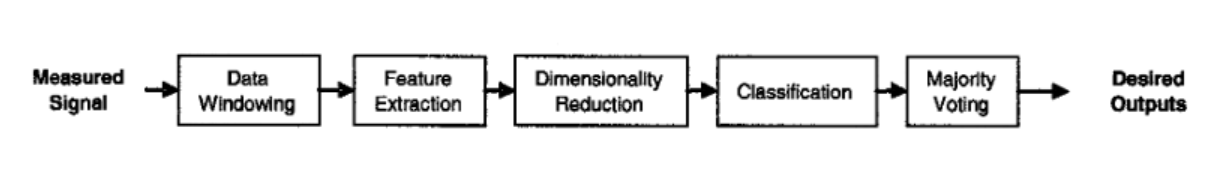
\includegraphics[width=15cm]{images/classificationPipeline.png}
    \caption{block diagram of the complete pipeline for posture classification using EMG signal \cite{ref:classification3}}
    \label{fig:classificationPipeline}
\end{figure}

This section shows different methods for the classification part the this pipeline. It is then possible to combine multiple classifier to enhance the prediction accuracy by using a majority vote upon the results of each classification.

We must also note that the reference article for posture classification often consider a very small number of EMG channels (up to a single channel) \cite{ref:classification1, ref:classification2}.


\subsubsection{Linear discriminant analysis classifier (LDAC)}


\subsubsection{Support vector machine (SVM)}
6 gestures
SVM for more than 2 classes (here, 6 classes): stategy one against all
First, they tried different sets of features with different SVM kernel
Then, they chose the set of feature that gave the best results and used Cuckoo Search Optimisation to optimize the SVM
Average correct classification rate of 96 \% for each kernel tested and 98.12\% for the optimized SVM with average standart deviation of 0.004 which is better than the smallest standard dev that they got without optimization
Good result but probably due to small number of gestures involved



\subsubsection{Convolutional neural network (CNN)}



\subsubsection{Multi-layer perception classifier (MLCP)}

Experimental results showed an average classification accuracy of 81.54%, 88.54%, and 94.19% for 8, 6, and 5 gesture-classes, respectively

Combined feature approach based on time–spectral analysis and CNN deep features.

A method that boost the accuracy of the EMG gesture recognition system.

A method that outperforms both the CNN and the time–spectral feature classifier.

Simple architecture which reduces the numbers of signals needed for training.

A method that achieves high accuracy with an acquisition device of one channel.

Proposed method reaches accuracy level greater than 80\% for 8 gestures

\subsubsection{Other methods}

The four classifiers that are described above are parts of the most popular ones for posture classification using EMG signals. However, there exists many other methods of classification which can be useful when doing combined classification. Among those techniques, we can cite fuzzy logic (FL), Bayesian classifier (BC) and neuro-fuzzy hybridization (NF) \cite{ref:classification3}.


\subsection{Gesture regression }

https://jneuroengrehab.biomedcentral.com/articles/10.1186/1743-0003-11-122
https://www.hindawi.com/journals/isrn/2012/604314/
https://pubmed.ncbi.nlm.nih.gov/22180516/




\end{document}